\chapter{Factory set-up}\label{ch:factory}

The Factory page holds everything about the plant that rarely changes: the production process, products
and their routes, machines, molds, shifts and calendar, and the policies that define a good schedule. It is
normally maintained by a plant engineer. Planners only read it, except for the occasional new holiday or a
policy tweak.

\section{How set-up changes work: drafts and versions}\label{sec:versions-drafts}

The set-up is \term{versioned}. You never edit the live configuration directly:

\begin{enumerate}
  \item Every change you make on any tab goes into a \term{draft}. The draft is kept in your browser, so it
        survives a page reload or a closed tab.
  \item A bar at the bottom of the page counts the unsaved changes and names the sections they touch.
  \item \ui{Save as v\textit{N}} turns the draft into a new, immutable version. You may give it an
        \ui{Effective from} date and a \ui{Change note}.
\end{enumerate}

\shotf[0.78\linewidth]{factory_draft_bar}{The draft bar after one change in the Process section.}{factory_draft_bar}

\begin{itemize}
  \item \textbf{Effective from} (blank = now): a version with a date applies only to planning periods that start
        on or after that date. Periods already planned keep the version they were created with. In the
        example, version~2 adds CNC lathe~3 from 7~December, so the period starting 23~November still uses
        version~1.
  \item \textbf{Validation.} If the draft is not consistent (for example a stock cap below the safety stock,
        or a product no machine can make), the bar shows ``\textit{n} error(s) to fix before saving'' and the
        save button is disabled. The first errors are listed so you can jump to them.
  \item \textbf{Discard} throws the draft away after a confirmation; the set-up goes back to the current
        version.
  \item \textbf{Leaving the page} with unsaved changes asks whether to stay or to leave and keep the draft.
        When you come back, the draft is reopened. If someone saved a newer version in the meantime, you are
        warned that saving the old draft would overwrite those changes, and you may drop it instead.
\end{itemize}

\begin{note}
A saved version never changes. This guarantees that a committed schedule can always be reproduced with
exactly the plant data it was planned with.
\end{note}

\section{Page overview and the Process tab}\label{sec:process}

\shot{factory_process}{The Factory page, Process tab.}{factory_process}

\begin{callouts}
  \item[1] \textbf{Set-up sections}, each with a count: Process (stages), Products, Machines, Molds, Shifts
           \& calendar, Policies, Versions.
  \item[2] \textbf{A stage card}: position and code (\code{1 · cast}), name, run size, number of machines and
           items, and tags such as \ui{molds}, \ui{24/7} or \ui{makes products} (the last stage).
  \item[3] \textbf{Transfer arrow}: the number is the minutes needed to move goods to the next stage
           (120~minutes before test and packing, because paint must cure). Hover an arrow to insert a stage
           there.
  \item[4] \textbf{Planning defaults} used when creating periods.
  \item[5] \textbf{Download JSON} exports the current set-up; the \ui{\dots} menu next to it renames the
           factory.
  \item[6] \textbf{Versions} lists every saved version (Section~\ref{sec:factory-versions}).
\end{callouts}

\subsection{Stages}

Every product passes the stages in the same order. Each stage works in \term{fixed-size runs} (every run
makes exactly that many units) and may have several parallel machines. Click a stage card to edit it:

\shotf[0.5\linewidth]{factory_stage_edit}{Editing the heat treatment stage.}{factory_stage_edit}

\begin{itemize}
  \item \ui{Display name}, \ui{Run size (units)} and \ui{Transfer to \dots\ (min)}.
  \item \ui{Position in the process}: \ui{Earlier}/\ui{Later} reorder the stages. Reordering changes the
        material flow; semi-finished codes and machine rates stay with their stage, so review them
        afterwards. A confirmation explains the consequences.
  \item \ui{Semi-finished codes made} at this stage and the \ui{Machines} of the stage, with a link to the
        Machines tab.
  \item \ui{Remove stage} deletes the stage together with its machines, semi-finished codes, molds and
        maintenance slots (the confirmation lists exactly what goes). Goods then flow straight from the
        previous stage to the next one.
\end{itemize}

\textbf{Adding a stage.} \ui{Add stage} (or the \ui{+} on an arrow) opens a dialog asking for the stage
name, its code (lower-case letters, digits or \_, fixed once saved), its position, run size and transfer
times, how many machines it gets (with a shared calendar, minutes per unit, fixed minutes per run and
changeover time; each machine can be fine-tuned later) and the new semi-finished codes leaving the stage. A
preview shows the process after adding. Rules that keep the model valid:

\begin{itemize}
  \item the plant needs at least two stages;
  \item a stage that uses molds (casting) cannot become the last stage;
  \item new semi-finished codes start with zero stock: if the floor already holds some, enter it as opening
        stock in each period.
\end{itemize}

\subsection{Planning defaults}

\begin{center}
\begin{tabularx}{\linewidth}{>{\bfseries}p{4.3cm}X}
\toprule
\rowcolor{white}Field & Meaning \\
\midrule
Period length (days) & Default length of a new planning period, 1--62 days (14 in the example). \\
Long-term look-ahead (days) & Orders due within this many days after a period are shown as ``after the period'' and may feed pull-ahead (28). \\
Default due time & Used when an imported order file gives a date without a time (16:00). \\
Time zone & The plant's time zone, fixed (UTC+07:00). All times in PlanWise are local plant time. \\
\bottomrule
\end{tabularx}
\end{center}

\section{Products and routes}\label{sec:products}

\shot{factory_products}{Products and the semi-finished codes they pass through.}{factory_products}

Each product lists its \term{route}: the semi-finished code it becomes at every stage. Products sharing a
code share that stock. In the example, silver and black front wheels share \code{F\_CAST}, \code{F\_HEAT}
and \code{F\_MACH}; they only differ from painting on. This is what lets the scheduler cast and heat-treat
in large common runs and decide the colour late.

\begin{itemize}
  \item \ui{Safety stock}: the finished-goods level the product should not fall below at the end-of-day
        checkpoints.
  \item \ui{Stock cap}: the warehouse limit; it must not be below the safety stock. The scheduler never plans
        finished stock above it; when the warehouse is full, test and packing waits.
  \item The \ui{Semi-finished codes} table below gives every code a display name and an optional
        \ui{Store capacity} (blank = unlimited buffer between stages).
\end{itemize}

Click a product row to edit it:

\shotf[0.5\linewidth]{factory_product_edit}{Editing a product: display name, safety stock, stock cap and the route.}{factory_product_edit}

\ui{Add product} creates a product by copying the route, safety stock and cap of an existing one; you then
adjust it. A new product or semi-finished code becomes makeable on every machine of the corresponding stage
at an average rate, so review the rates under Machines. \ui{Delete product} removes it with its rates and
changeovers on every machine; codes nothing uses any more are removed too. The plant needs at least one
product.

\section{Machines}\label{sec:machines}

\shot{factory_machines}{Machines grouped by stage, with calendar, items made, rates and weekly service.}{factory_machines}

The table lists every machine by stage with its \ui{Calendar} (\ui{Shifts} or \ui{24/7}), the items it
\ui{Makes}, its \ui{Min/unit}, its \ui{Fixed/run} time and the number of weekly service slots. Click a
machine to edit it:

\shotf[0.6\linewidth]{factory_machine_edit}{Editing CNC lathe 1: rates and the changeover matrix.}{factory_machine_edit}

\begin{description}[style=nextline, leftmargin=1.2em, font=\bfseries\color{brand}]
  \item[Display name] The name shown in work orders and calendars (the code, e.g.\ \code{CNC\_1}, is fixed).
  \item[Calendar] \ui{By shift}: the machine works the daily shifts (Section~\ref{sec:calendar}).
        \ui{Continuous 24/7 (furnace)}: it runs around the clock and only stops on rest days, holidays and
        maintenance.
  \item[Fixed time per run (min)] Time added to every run whatever its size (loading, warm-up). For a furnace
        the whole cycle is fixed time: 480 minutes per load.
  \item[Mold change at least (min)] For casting machines: minimum time for swapping molds.
  \item[Items and rates] Which semi-finished codes the machine can make (\ui{Made here}) and the minutes per
        unit for each. \ui{One run} shows the resulting run time:
        \[ \text{run time} = \text{run size} \times \text{minutes per unit} + \text{fixed time}. \]
        An item only this machine makes cannot be switched off.
  \item[Changeover times (min)] A matrix: the row is what the machine did last (or its state), the column is
        what it switches to. Darker cells cost more time; the diagonal (same item) needs no changeover. The
        \ui{Start} row is the changeover from the initial state at the start of a period; an \ui{After
        service} row (casting) is the state after mold maintenance.
  \item[Weekly planned maintenance] Shown here, edited under Shifts \& calendar.
\end{description}

\ui{Duplicate} creates a new machine with the same rates, changeovers and calendar (recurring maintenance is
not copied) --- the usual way to add a parallel machine. \ui{Delete machine} is refused when it is the
stage's only machine or the only one that makes some item.

\section{Molds}\label{sec:molds}

\shot{factory_molds}{Casting molds with their cycle limits.}{factory_molds}

Molds are shared by the machines of a stage; each casting run needs one mold of its item. After a number of
cycles (\ui{Cycle limit}) a mold must be serviced (\ui{Service (min)}) before it can cast again; the
scheduler inserts that maintenance automatically and you will see it on the Gantt chart and in the work
orders (\ui{mold service}). \ui{Cavities} is the number of parts per cycle. \ui{After service} is the
machine state after mold service --- a row of the changeover matrix (here \code{CLEAN}, which needs 30~minutes
before the next run).

How many cycles each mold has already used is not set-up data: it is entered per period, with the opening
stock (Section~\ref{sec:opening}). Each cast item needs at least one mold.

\section{Shifts and calendar}\label{sec:calendar}

\begin{figure}[H]\centering
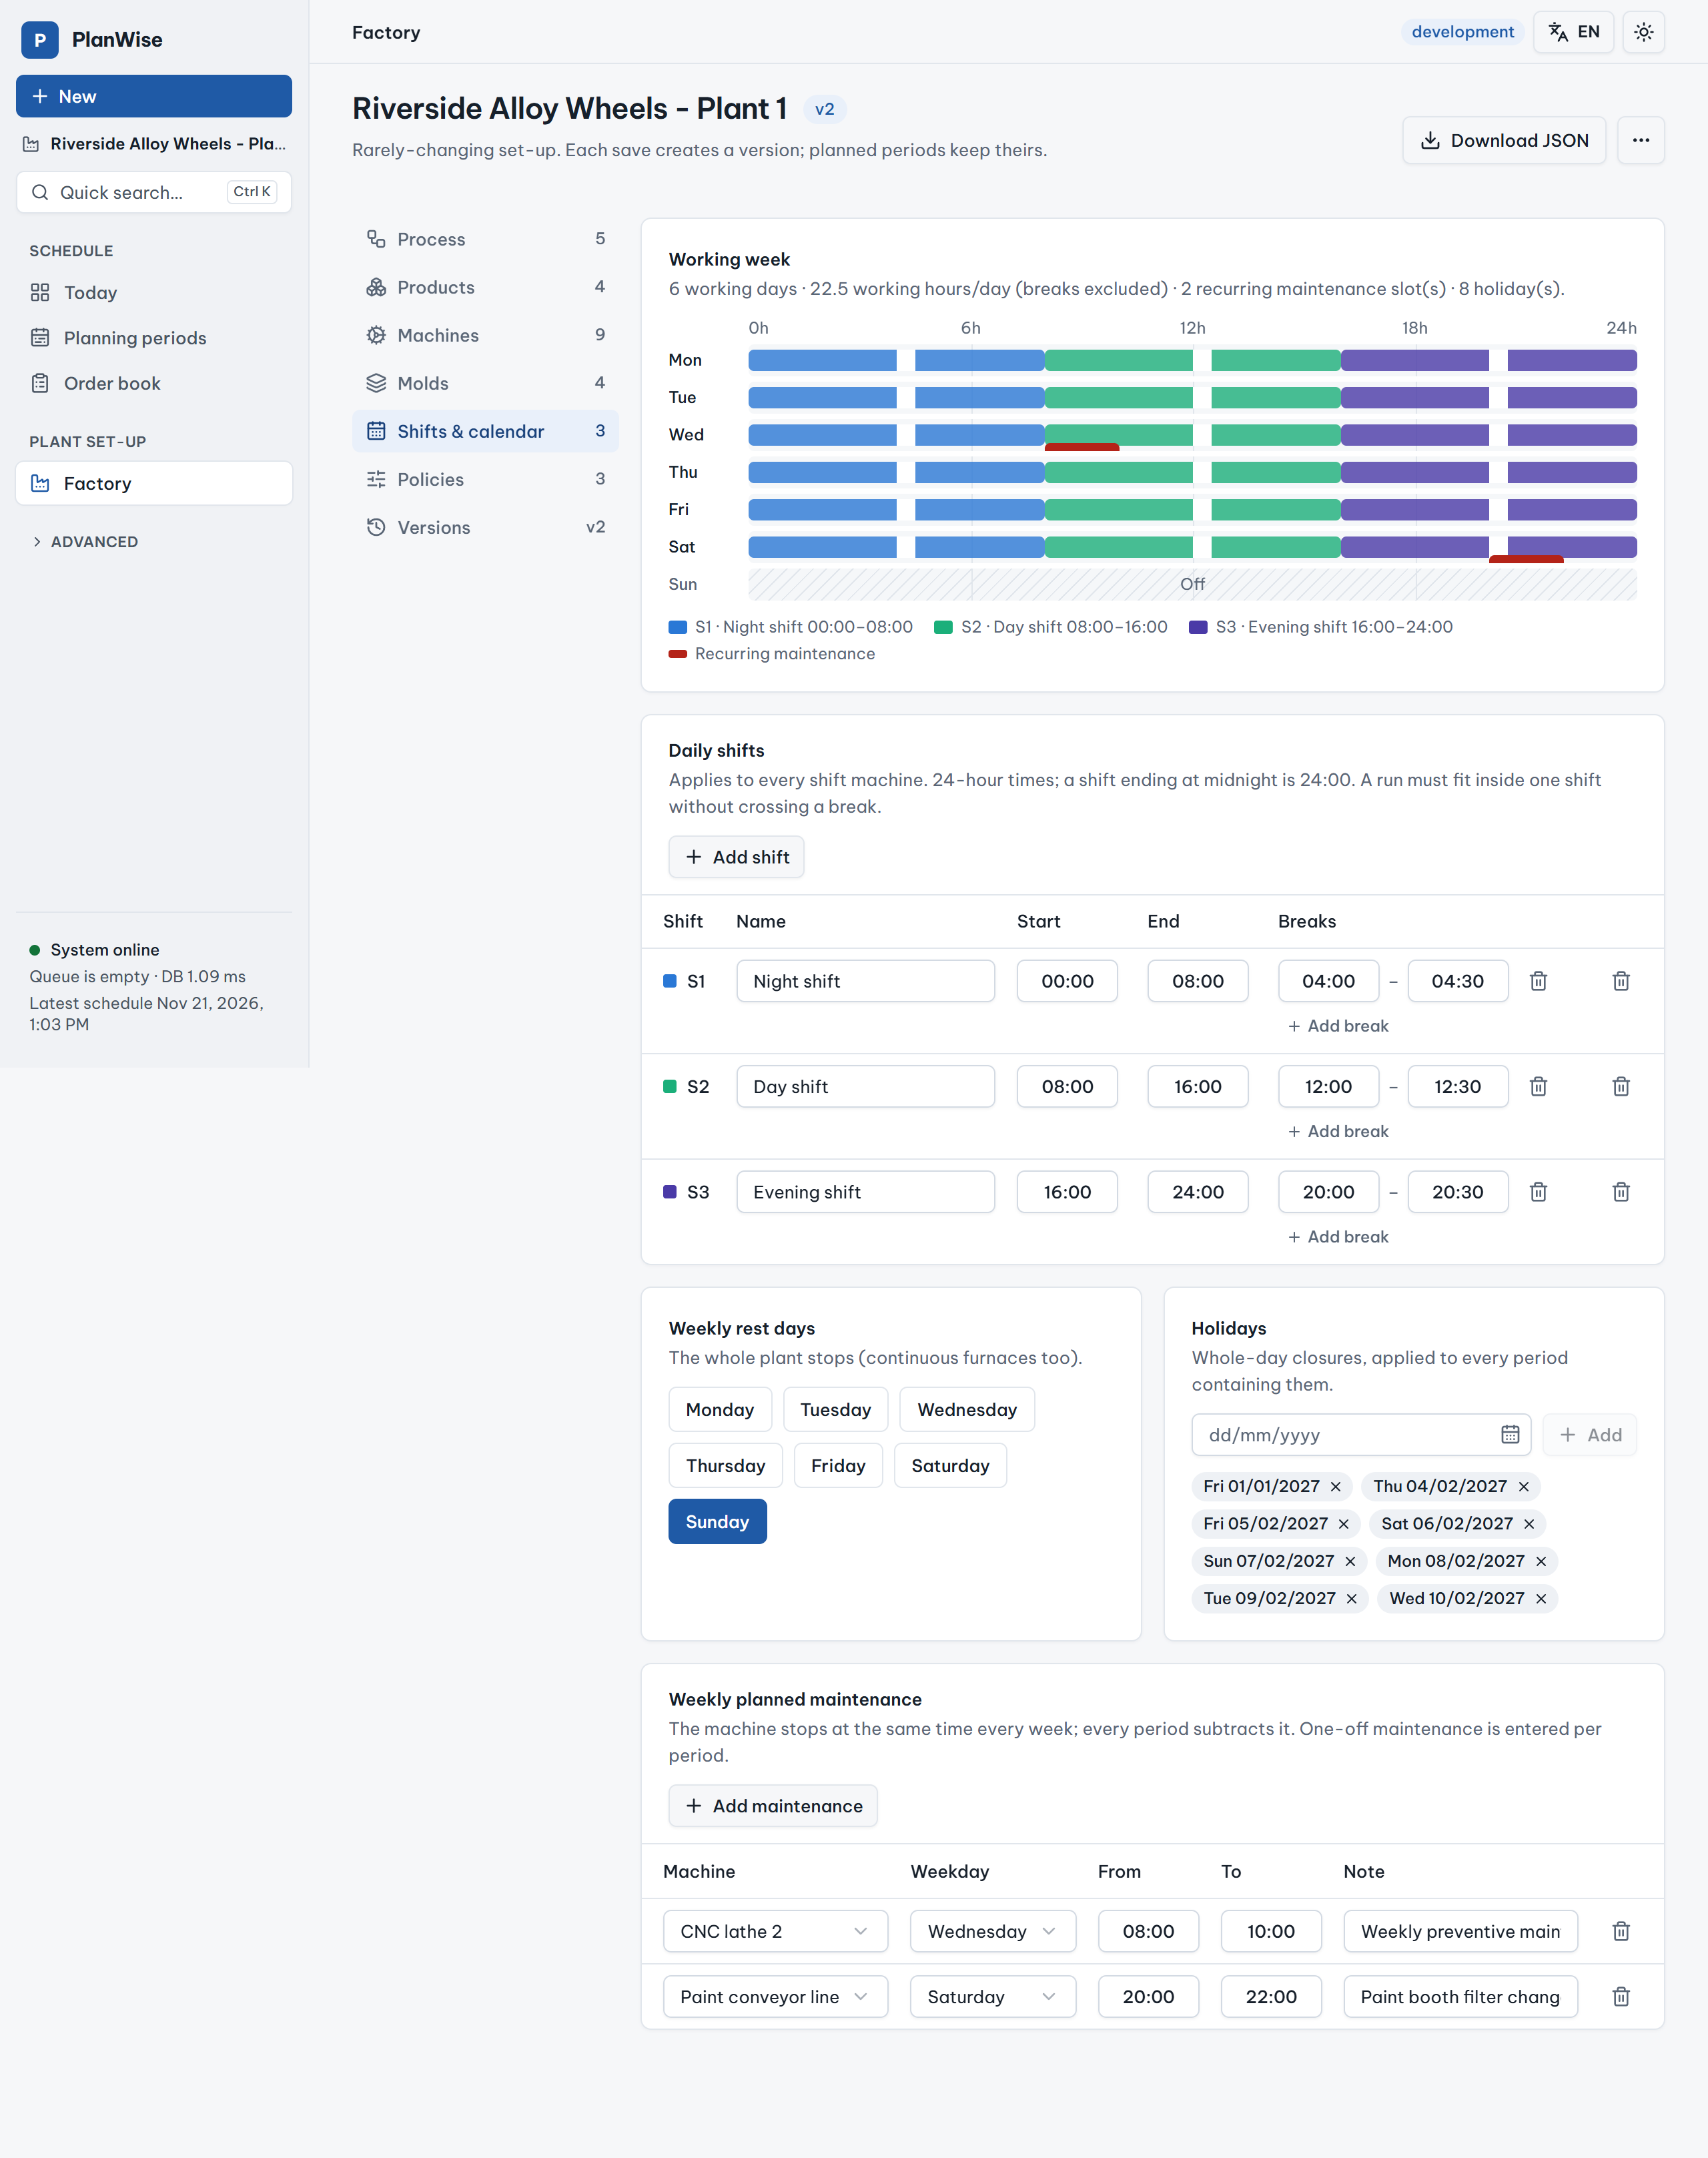
\includegraphics[width=0.62\linewidth]{factory_calendar}
\caption{Shifts \& calendar: week grid, daily shifts, rest days, holidays and weekly maintenance.}\label{fig:factory_calendar}
\end{figure}

\begin{description}[style=nextline, leftmargin=1.2em, font=\bfseries\color{brand}]
  \item[Working week grid] A visual summary of a week: shifts per day, breaks, rest days and recurring
        maintenance. Overlapping shifts are flagged.
  \item[Daily shifts] Apply to every machine on a shift calendar. Times are 24-hour; a shift ending at
        midnight ends at 24:00. Each shift can have breaks. \textbf{A run must fit inside one shift without
        crossing a break}, which is why breaks influence how long runs can be. The example uses three
        eight-hour shifts (night 00:00--08:00, day 08:00--16:00, evening 16:00--24:00) with a 30-minute meal
        break each.
  \item[Weekly rest days] The whole plant stops, continuous furnaces included (Sunday in the example).
  \item[Holidays] Whole-day closures, applied to every period that contains them (New Year and Lunar New
        Year in the example).
  \item[Weekly planned maintenance] A machine stops at the same time every week (weekday, from, to, note),
        and every period subtracts that time. One-off maintenance belongs to a period instead
        (Section~\ref{sec:period-calendar}).
\end{description}

\section{Policies}\label{sec:policies}

A policy decides which schedule counts as better. The score of a schedule is
\[ \text{score} = \sum_{\text{terms}} \text{weight} \times \text{objective value}, \qquad \text{lower is better}. \]
Terms marked \ui{Strictly first} are multiplied by a large scale factor (here one million) before summing, so
they always dominate the others: two schedules are first compared on those terms, and the others only break
ties. Each period picks one policy; the default is marked with a star.

\shot{factory_policies}{The default policy ``On-time delivery first'' with its weights.}{factory_policies}

For each objective term you set a \ui{Weight}; \ui{Share} shows its share of the total weight, and the
checkbox makes it strictly first (only possible with a weight above zero). \ui{Make default},
\ui{Duplicate} and delete are available per policy; the default policy cannot be deleted.

\begin{center}
\begin{tabularx}{\linewidth}{>{\bfseries}p{4.4cm}X}
\toprule
\rowcolor{white}Objective term & What is measured \\
\midrule
Weighted tardiness & Minutes late $\times$ order priority, summed over orders. \\
Safety-stock shortfall & Units below safety stock, summed over the end-of-day checkpoints. \\
Makespan & Minutes from the period start to the end of the last run. \\
Non-productive minutes & Minutes of opened machine shifts not spent processing (idle, setup, maintenance). \\
Setup minutes & Total changeover minutes between items. \\
Mold maintenance minutes & Total mold service minutes. \\
Idle minutes & Machine minutes left unused inside opened shifts. \\
Pulled-ahead units & Units made ahead for orders due after the period. \\
Pull-ahead options & Runs (options) made ahead for after-period orders. \\
Stock above safety & Units held above safety stock at the checkpoints. \\
Semi-finished left at end & Semi-finished units left at the end of the period. \\
\bottomrule
\end{tabularx}
\end{center}

The example plant has three policies: \textbf{On-time delivery first} (default; weighted tardiness and
safety-stock shortfall strictly first), \textbf{Balanced} (one weighted sum) and \textbf{Lowest running cost}
(for slack weeks: fewer shifts, setups and idle time; small delays tolerated).

\begin{note}
Weights belong to the factory. The \ui{Service first / Balanced / Cost first} switch on the Options tab
(Section~\ref{sec:ranking}) only changes the \emph{order} in which the same weighted terms are compared, not the
weights.
\end{note}

\section{Versions}\label{sec:factory-versions}

\shot{factory_versions}{Two versions: v2 (CNC lathe 3, effective 7 December) and v1 (imported).}{factory_versions}

Every save creates an immutable version. Each row shows the version number, \ui{latest}, the effective date,
when and by whom it was saved, the change note, how many periods use it, and the number of changes. Expand a
version to see its changes, then:

\begin{itemize}
  \item \ui{Compare with the current one} shows a side-by-side list: left the value in the old version, right
        the current value (including your unsaved draft);
  \item \ui{Restore into the draft} loads that version into the draft so you can review and save it as a new
        version.
\end{itemize}

\shot{factory_version_compare}{Comparing version 1 with the current set-up.}{factory_version_compare}

\begin{tip}
When a newer version becomes applicable to an existing period (for example you saved a version effective
from a date inside the period), the period header shows ``Factory set-up v\textit{N} available\dots''. Click it
and confirm \ui{Use v\textit{N}} to move the period to that version; its inputs are then checked again.
\end{tip}
